\documentclass[12pt,a4paper]{report}
\usepackage[utf8]{inputenc}
\usepackage[T1]{fontenc}
\usepackage[french]{babel}
\usepackage{graphicx}
\usepackage{hyperref}
\usepackage{geometry}
\usepackage{blindtext}
\usepackage{enumitem}
\geometry{margin=2.5cm}
\usepackage{fancyhdr}
\usepackage{titlesec}
\usepackage{tocloft}
\usepackage{setspace}
\usepackage{newunicodechar}
\newunicodechar{─}{-}
\usepackage{caption}
\usepackage{subcaption}
\usepackage[utf8]{inputenc}
\usepackage{enumitem}

\usepackage{float} % Pour le positionnement des figures
\usepackage{graphicx} % Pour les images
\usepackage{minted}  % Pour le code coloré
\usepackage{listings}  % Pour les blocs verbatim
\usepackage[utf8]{inputenc}
\usepackage{graphicx}

\begin{document}
% === PAGE DE GARDE ===
\begin{titlepage}
    \thispagestyle{empty}  % Aucune numérotation sur cette page

\vspace*{-1cm}  % Ajuste si besoin pour remonter les logos

\begin{figure}[t]
    \begin{minipage}{0.05\textwidth}
        \raggedright
        \includegraphics[width=2.5in]{logo.png}
    \end{minipage}
    \hfill
    \begin{minipage}{0.4\textwidth}
        \raggedleft
        \includegraphics[width=3in]{logo1.jpg}
    \end{minipage}
\end{figure}

\vspace{1cm}  % Espace sous les logos si tu veux du contenu ensuite
    \centering
    \vspace*{1.5cm}
    {\Huge\bfseries Application de Gestion de Photos\par}
     \vspace{0.5cm}
    {\Large\bfseries Photo Gallery \par}
    \vspace{3cm}
    {\Large Rapport de projet\par}
    \vspace{1cm}
    {\large Préparé par : Es-soualhi Abdellah, Aymane Ennaqadi et Akram hamimou\par}
    \vspace{0.5cm}
    {\large Encadré par : Mr.Yves Frédéric EBOBISSE DJENE \par}
    \vfill
    {\large EMSI\\
    3IIR12\\}
    \vspace{1cm}


    \textit{Année universitaire 2024/2025} 
\end{titlepage}

\pagenumbering{roman}
\tableofcontents
\newpage

\chapter*{Remerciements}
\addcontentsline{toc}{chapter}{Remerciements}

\chapter*{Résumé}
\addcontentsline{toc}{chapter}{Résumé}

Ce projet consiste en la conception et le développement d’une application web innovante dédiée à la gestion et au partage de recettes culinaires, réalisée avec le framework Django. L’application permet aux utilisateurs de s’inscrire, de créer, consulter, modifier et supprimer des recettes, d’ajouter des ingrédients, de spécifier les étapes de préparation, de joindre des images, et de catégoriser les recettes par type de plat, difficulté, cuisine et tags. Les utilisateurs peuvent également commenter les recettes, les ajouter à leurs favoris, et interagir via un module de blog culinaire. Un espace administrateur offre la gestion des utilisateurs, des ingrédients, des tags, ainsi que la modération des contenus. L’ergonomie, la sécurité et la convivialité sont au cœur du développement afin d’offrir une expérience utilisateur optimale. Ce rapport détaille l’ensemble du processus, de l’analyse des besoins à la mise en œuvre technique, en passant par la conception, la modélisation et les choix technologiques, dans le but de favoriser le partage, la découverte et l’apprentissage autour de la cuisine.
\chapter*{Abstract}
\addcontentsline{toc}{chapter}{Abstract}

This project involves the design and development of an innovative web application dedicated to the management and sharing of culinary recipes, built with the Django framework. The application allows users to register, create, view, edit, and delete recipes, add ingredients, specify preparation steps, upload images, and categorize recipes by meal type, difficulty, cuisine, and tags. Users can also comment on recipes, add them to their favorites, and interact through a culinary blog module. An administrator area provides management of users, ingredients, tags, and content moderation. Usability, security, and user-friendliness are at the heart of the development to ensure an optimal user experience. This report details the entire process, from requirements analysis to technical implementation, including design, modeling, and technological choices, with the aim of fostering sharing, discovery, and learning around cooking.
\newpage
\listoffigures
\newpage
\pagenumbering{arabic}

\chapter*{Introduction générale}
\addcontentsline{toc}{chapter}{Introduction générale}

\begin{quote}
    \emph{« La cuisine est le seul art qui nourrit. »} \\
    \hfill --- Pierre Dac
\end{quote}

Aujourd’hui, la cuisine occupe une place importante dans la vie de nombreuses personnes. Elle permet non seulement de se nourrir, mais aussi de partager des moments conviviaux, de découvrir de nouvelles cultures et d’exprimer sa créativité. Avec l’évolution des technologies et l’accès facile à Internet, il est devenu courant de chercher, partager et commenter des recettes en ligne. Les plateformes de partage de recettes sont ainsi devenues des outils précieux pour les passionnés de cuisine, les familles et même les professionnels.

Dans ce contexte, nous avons choisi de réaliser un projet qui répond à ce besoin croissant de partage et d’organisation des recettes culinaires. Notre application web, développée avec le framework Django, permet à chaque utilisateur de créer un compte, d’ajouter ses propres recettes, de consulter celles des autres, de laisser des commentaires et de marquer ses recettes préférées. L’application propose aussi un espace blog pour publier des articles culinaires, des astuces ou des expériences personnelles.

L’objectif principal de ce projet est de faciliter l’accès à une grande variété de recettes, de permettre à chacun de partager ses idées et de découvrir de nouvelles saveurs. Nous avons également accordé une grande importance à la simplicité d’utilisation, à la sécurité des données et à la convivialité de l’interface. Ce rapport présente toutes les étapes de la réalisation du projet, depuis l’analyse des besoins jusqu’à la mise en œuvre technique, en passant par la conception, la modélisation et les choix technologiques. Nous espérons que cette plateforme contribuera à rendre la cuisine encore plus accessible, interactive et agréable pour tous.

% Chapitre 1
\chapter{Contexte du projet}
\section*{Introduction}
\addcontentsline{toc}{section}{Introduction}

La cuisine occupe une place essentielle dans la vie quotidienne de chacun. Elle permet non seulement de se nourrir, mais aussi de partager des moments conviviaux, de découvrir de nouvelles cultures et d’exprimer sa créativité. Avec l’évolution des technologies et l’accès généralisé à Internet, de plus en plus de personnes souhaitent partager leurs recettes, apprendre de nouvelles techniques et échanger autour de leur passion pour la gastronomie. Dans ce contexte, il devient pertinent de proposer une solution numérique qui facilite la gestion, l’organisation et le partage de recettes culinaires. Ce chapitre présente le contexte général du projet, ses motivations et les besoins auxquels il cherche à répondre.

\section{Présentation générale du projet}

Le projet que nous avons réalisé consiste à développer une application web dédiée à la gestion et au partage de recettes de cuisine. Cette plateforme permet à chaque utilisateur de créer un compte personnel afin d’ajouter ses propres recettes, de consulter celles partagées par d’autres membres, et de découvrir de nouvelles idées culinaires. L’application offre la possibilité de détailler chaque recette avec une liste d’ingrédients, des étapes de préparation, une photo, ainsi que des informations sur la difficulté, le type de plat ou la cuisine d’origine.

En plus de la gestion des recettes, l’utilisateur peut commenter les réalisations, ajouter ses recettes préférées à une liste de favoris, et participer à la vie de la communauté grâce à un module de blog culinaire. Un espace administrateur est également prévu pour gérer les utilisateurs, les ingrédients, les tags et assurer la modération des contenus publiés sur la plateforme.

L’objectif principal de ce projet est de proposer un outil simple, convivial et sécurisé, qui facilite le partage, l’organisation et la découverte de recettes, tout en favorisant l’échange et l’apprentissage autour de la cuisine.
\newpage
\subsection{Problématique}

De nos jours, il existe une multitude de recettes de cuisine disponibles sur Internet, mais il n’est pas toujours facile de les organiser, de retrouver celles qui nous plaisent ou de partager ses propres créations avec une communauté. Beaucoup de plateformes sont limitées, soit par leur manque de fonctionnalités, soit par une interface peu intuitive, ce qui peut décourager les utilisateurs à participer activement.

De plus, la gestion des ingrédients, des étapes de préparation, des catégories ou encore l’interaction entre les membres (commentaires, favoris, blogs) sont souvent absentes ou incomplètes. Il devient alors difficile pour un passionné de cuisine de centraliser ses recettes, d’échanger avec d’autres utilisateurs ou de découvrir de nouvelles idées de manière simple et agréable.

Face à ces constats, il est nécessaire de concevoir une application web qui centralise toutes ces fonctionnalités, tout en restant facile à utiliser, moderne et accessible à tous.
\subsection{Étude de l'existant}

Aujourd’hui, plusieurs sites et applications proposent le partage de recettes de cuisine, comme Marmiton, 750g ou encore Cookpad. Ces plateformes permettent aux utilisateurs de consulter un grand nombre de recettes, de publier leurs propres créations et parfois d’interagir via des commentaires ou des notes. Cependant, ces solutions présentent souvent certaines limites : certaines fonctionnalités avancées, comme la gestion détaillée des ingrédients, la personnalisation des étapes de préparation, ou la possibilité de créer un blog culinaire personnel, sont parfois absentes ou réservées à une partie des utilisateurs.

De plus, l’ergonomie et la simplicité d’utilisation ne sont pas toujours au rendez-vous, ce qui peut rendre l’expérience moins agréable, surtout pour les nouveaux utilisateurs. Enfin, la gestion de la confidentialité, la modération des contenus et la sécurité des données ne sont pas toujours mises en avant.

Face à ces constats, il apparaît pertinent de proposer une nouvelle application qui reprend les points forts des solutions existantes tout en apportant des améliorations en termes de fonctionnalités, d’ergonomie et de sécurité, afin de mieux répondre aux attentes des passionnés de cuisine.
\section{Objectifs du projet}

L’objectif principal de ce projet est de concevoir et de développer une application web moderne et intuitive permettant la gestion et le partage de recettes de cuisine. Cette plateforme vise à répondre aux besoins des passionnés de cuisine, qu’ils soient amateurs ou professionnels, en leur offrant un espace convivial pour organiser, publier et découvrir des recettes variées.

Les objectifs spécifiques du projet sont les suivants :
\begin{itemize}[label=•]
    \item Permettre à chaque utilisateur de créer un compte personnel et de gérer ses propres recettes.
    \item Offrir la possibilité d’ajouter, de modifier, de supprimer et de consulter des recettes détaillées (ingrédients, étapes, photos, catégories, etc.).
    \item Faciliter la recherche et la découverte de nouvelles recettes grâce à des filtres par type de plat, difficulté, cuisine, ou tags.
    \item Favoriser l’interaction entre les membres via les commentaires, les favoris et un module de blog culinaire.
    \item Mettre à disposition un espace d’administration pour la gestion des utilisateurs, des ingrédients, des tags et la modération des contenus.
    \item Garantir la sécurité des données et la confidentialité des informations personnelles.
    \item Proposer une interface simple, ergonomique et agréable à utiliser, accessible sur différents supports (ordinateur, tablette, smartphone).
\end{itemize}

En atteignant ces objectifs, le projet ambitionne de créer une communauté active autour de la cuisine, où le partage, l’apprentissage et la découverte sont au cœur de l’expérience utilisateur.
\section{Solution proposée}

Pour répondre aux besoins identifiés et aux objectifs fixés, la solution proposée consiste à développer une application web moderne et intuitive, basée sur le framework Django. Cette plateforme permettra à chaque utilisateur de créer un compte, de gérer ses propres recettes, de consulter et de commenter celles des autres, et de participer à la vie de la communauté culinaire.

L’application offrira les fonctionnalités suivantes :
\begin{itemize}[label=•]
    \item Création, modification, suppression et consultation de recettes détaillées, avec gestion des ingrédients, des étapes de préparation, des photos, des catégories et des tags.
    \item Recherche et filtrage des recettes selon différents critères (type de plat, difficulté, cuisine, etc.).
    \item Ajout de recettes aux favoris pour un accès rapide et personnalisé.
    \item Possibilité de commenter les recettes et d’interagir avec les autres membres.
    \item Module de blog culinaire pour partager des articles, des astuces ou des expériences personnelles.
    \item Espace d’administration pour la gestion des utilisateurs, des ingrédients, des tags et la modération des contenus publiés.
    \item Interface ergonomique, responsive et sécurisée, accessible sur ordinateur, tablette et smartphone.
\end{itemize}

Grâce à cette solution, l’utilisateur pourra organiser facilement ses recettes, découvrir de nouvelles idées culinaires, partager ses créations et échanger avec une communauté active, le tout dans un environnement convivial et sécurisé.
\section*{Conclusion}
\addcontentsline{toc}{section}{Conclusion}

Ce premier chapitre a permis de présenter le contexte général du projet, d’identifier les besoins des utilisateurs et de mettre en avant les limites des solutions existantes. Nous avons également défini les objectifs à atteindre et proposé une solution adaptée, centrée sur la simplicité, l’ergonomie et la richesse fonctionnelle. La plateforme envisagée vise à faciliter la gestion et le partage de recettes de cuisine, tout en favorisant l’échange et la découverte au sein d’une communauté active. Les chapitres suivants détailleront l’étude des besoins, l’analyse, la conception et la réalisation technique de cette application web.

% Chapitre 2
\chapter{Étude des besoins}
\section*{Introduction}
\addcontentsline{toc}{section}{Introduction}

Après avoir présenté le contexte général du projet et défini les objectifs à atteindre, il est essentiel d’identifier précisément les besoins auxquels l’application doit répondre. Cette étape permet de s’assurer que la solution proposée sera en adéquation avec les attentes des utilisateurs et les exigences fonctionnelles et techniques du projet. Ce chapitre présente l’ensemble des besoins fonctionnels et non-fonctionnels, ainsi que la description des différents acteurs qui interagiront avec la plateforme.
\section{Besoins fonctionnels}

Les besoins fonctionnels décrivent l’ensemble des fonctionnalités que l’application doit offrir pour répondre aux attentes des utilisateurs. Pour ce projet de gestion de recettes de cuisine, les besoins fonctionnels identifiés sont les suivants :

\begin{itemize}[label=•]
    \item Permettre à un utilisateur de créer un compte, de se connecter et de gérer son profil.
    \item Ajouter, modifier, supprimer et consulter des recettes de cuisine.
    \item Associer à chaque recette une liste d’ingrédients, des étapes de préparation, une photo, un niveau de difficulté, un type de plat, une cuisine d’origine et des tags.
    \item Rechercher et filtrer les recettes selon différents critères (ingrédients, type de plat, difficulté, cuisine, tags, etc.).
    \item Ajouter des recettes à une liste de favoris pour un accès rapide.
    \item Commenter les recettes et consulter les commentaires des autres utilisateurs.
    \item Gérer un module de blog pour publier des articles culinaires, des astuces ou des expériences personnelles.
    \item Pour l’administrateur : gérer les utilisateurs, les ingrédients, les tags, les recettes et modérer les contenus publiés sur la plateforme.
\end{itemize}

Ces besoins fonctionnels constituent la base des principales interactions entre les utilisateurs et l’application, et garantissent une expérience riche et complète autour du partage de recettes de cuisine.
\section{Besoins non-fonctionnels}

Les besoins non-fonctionnels concernent les exigences de qualité, de performance et de sécurité que l’application doit respecter, en complément des fonctionnalités principales. Pour ce projet, les besoins non-fonctionnels identifiés sont les suivants :

\begin{itemize}
    \item \textbf{Ergonomie et simplicité d’utilisation} : l’interface doit être intuitive, agréable et facile à prendre en main, même pour des utilisateurs débutants.
    \item \textbf{Performance} : l’application doit offrir des temps de réponse rapides, même en cas de forte affluence ou de nombreuses recettes enregistrées.
    \item \textbf{Sécurité} : les données personnelles des utilisateurs doivent être protégées, et l’accès aux fonctionnalités sensibles (administration, modification, suppression) doit être sécurisé.
    \item \textbf{Confidentialité} : les informations privées des utilisateurs ne doivent pas être accessibles aux autres membres sans autorisation.
    \item \textbf{Compatibilité} : l’application doit être accessible depuis différents appareils (ordinateurs, tablettes, smartphones) et navigateurs web courants.
    \item \textbf{Maintenabilité} : le code doit être structuré et documenté pour faciliter les évolutions et la correction d’éventuels bugs.
    \item \textbf{Scalabilité} : la solution doit pouvoir évoluer pour accueillir un nombre croissant d’utilisateurs et de recettes sans perte de performance.
    \item \textbf{Sauvegarde des données} : il doit être possible de sauvegarder et de restaurer les données importantes de l’application.
\end{itemize}

Le respect de ces besoins non-fonctionnels est essentiel pour garantir la qualité, la fiabilité et la pérennité de la plateforme.
\section{Description des acteurs}

L’application de gestion de recettes de cuisine fait intervenir plusieurs types d’acteurs, chacun ayant des rôles et des droits spécifiques :

\begin{itemize}
    \item \textbf{Visiteur} : toute personne accédant à la plateforme sans être connectée. Le visiteur peut consulter les recettes publiques, lire les articles du blog et effectuer des recherches, mais il ne peut pas ajouter de contenu ni interagir avec la communauté.
    \item \textbf{Utilisateur inscrit} : après création d’un compte, l’utilisateur peut ajouter, modifier et supprimer ses propres recettes, commenter celles des autres, ajouter des recettes à ses favoris, gérer son profil et publier des articles sur le blog.
    \item \textbf{Administrateur} : il dispose de droits étendus sur la plateforme. L’administrateur peut gérer l’ensemble des utilisateurs, valider ou supprimer des recettes, modérer les commentaires et les articles du blog, gérer les ingrédients, les tags et assurer la sécurité et la bonne organisation du site.
\end{itemize}

Chaque acteur joue un rôle essentiel dans le fonctionnement et l’animation de la plateforme, contribuant ainsi à la richesse et à la diversité des contenus proposés.
\section*{Conclusion}
\addcontentsline{toc}{section}{Conclusion}


Ce chapitre a permis d’identifier et de détailler l’ensemble des besoins auxquels l’application doit répondre, qu’ils soient fonctionnels ou non-fonctionnels. Nous avons également présenté les différents acteurs qui interagiront avec la plateforme, chacun ayant des rôles et des droits spécifiques. Cette analyse approfondie des besoins constitue une base solide pour la suite du projet, en orientant les choix de conception et de développement afin de garantir une solution adaptée, efficace et conviviale. Le chapitre suivant portera sur l’analyse et la conception de l’application, en s’appuyant sur les besoins exprimés ici.
\newpage
% Chapitre 3
\chapter{Analyse et conception}
\section*{Introduction}
\addcontentsline{toc}{section}{Introduction}

Après avoir défini les besoins fonctionnels et non-fonctionnels de l’application, il est essentiel de passer à l’étape d’analyse et de conception. Cette phase permet de structurer le projet, de modéliser les différentes entités et leurs relations, et de choisir les outils et méthodes adaptés pour garantir la réussite du développement. Ce chapitre présente les outils de modélisation utilisés, les diagrammes de cas d’utilisation, les diagrammes de séquence ainsi que le diagramme de classes, qui constituent la base de l’architecture de l’application.

\section{Outils de modélisation utilisés}

Pour concevoir et structurer l’architecture de l’application, il est important d’utiliser des outils de modélisation adaptés. Dans le cadre de ce projet, nous avons utilisé le logiciel \textbf{Astah UML} pour réaliser l’ensemble des diagrammes nécessaires à la conception.

Astah UML permet de créer facilement différents types de diagrammes, notamment :
\begin{itemize}
    \item \textbf{Diagramme de cas d’utilisation} : pour représenter les interactions entre les utilisateurs (acteurs) et l’application, et identifier les principales fonctionnalités offertes.
    \item \textbf{Diagrammes de séquence} : pour décrire le déroulement des échanges entre les acteurs et le système lors de scénarios précis.
    \item \textbf{Diagramme de classes} : pour modéliser les entités principales de l’application, leurs attributs, leurs méthodes et les relations entre elles.
\end{itemize}

L’utilisation d’Astah UML a permis de produire des schémas clairs et structurés, facilitant ainsi la compréhension et la mise en œuvre du projet.
\addcontentsline{toc}{section}{Conclusion}
\begin{figure}[H]
    \centering
    \includegraphics[width=0.2\textwidth]{download.jpg}
    \caption{Logo du logiciel Astah UML}
    \label{fig:astah_uml}
\end{figure}

\section{Diagramme de cas d’utilisation}
\subsection{Diagramme de cas d’utilisation : Utilisateur invité et utilisateur inscrit}

\begin{figure}[H]
    \centering
    \includegraphics[width=0.95\textwidth]{Diagramme de cas d'ustilisation.jpg}
    \caption{Diagramme de cas d’utilisation – Utilisateur invité et utilisateur inscrit}
    \label{fig:usecase_invite_inscrit}
\end{figure}

Ce diagramme illustre les différentes interactions possibles entre l’application et deux types d’utilisateurs : l’utilisateur invité (non connecté) et l’utilisateur inscrit (ayant un compte et connecté).

\begin{itemize}
    \item \textbf{Utilisateur invité} : il peut parcourir les recettes publiques, consulter les détails d’une recette, voir les conseils de cuisine, lire les articles de blog, contacter le support, et s’inscrire sur la plateforme. Certaines actions, comme voir les détails d’une recette ou accéder à des fonctionnalités avancées, nécessitent de se connecter.
    \item \textbf{Utilisateur inscrit} : en plus des droits de l’utilisateur invité, il peut créer, modifier, supprimer ses propres recettes, ajouter une image à une recette, définir la visibilité de ses recettes, ajouter ou retirer une recette de ses favoris, voir ses recettes favorites, commenter les recettes, gérer son profil, télécharger un avatar, et gérer ses propres photos (ajout, suppression, favoris).
\end{itemize}

Le diagramme met en évidence les relations entre les différents cas d’utilisation (<<include>>, <<extend>>) et la nécessité de se connecter pour accéder à certaines fonctionnalités. Il permet ainsi de visualiser clairement les possibilités offertes à chaque type d’utilisateur sur la plateforme.
\subsection{Diagramme de cas d’utilisation : Gestion des utilisateurs (Administrateur)}

Il est important de noter que l’administrateur hérite de l’ensemble des droits et fonctionnalités attribués à un utilisateur inscrit. L’administrateur peut donc également effectuer toutes les actions accessibles aux utilisateurs inscrits, telles que la création, la modification et la suppression de recettes, la gestion de son profil, l’ajout de commentaires, ou encore la gestion de ses favoris. Ce principe d’héritage permet à l’administrateur d’avoir une maîtrise complète sur la plateforme, tout en participant activement à la vie de la communauté comme un utilisateur classique.

\begin{figure}[H]
    \centering
    \includegraphics[width=0.95\textwidth]{admin1.jpg}
    \caption{Diagramme de cas d’utilisation – Gestion des utilisateurs par l’administrateur}
    \label{fig:usecase_admin_utilisateur}
\end{figure}

Ce diagramme représente le package de cas d’utilisation dédié à la gestion des utilisateurs, accessible uniquement à l’administrateur de la plateforme. L’administrateur dispose de droits avancés lui permettant d’assurer la modération et la bonne organisation du site.

Les principales fonctionnalités regroupées dans ce package sont:
\begin{itemize}
    \item \textbf{Gérer les utilisateurs} : action principale qui regroupe toutes les opérations de gestion sur les comptes utilisateurs.
    \item \textbf{Supprimer un utilisateur} : possibilité de retirer définitivement un utilisateur de la plateforme.
    \item \textbf{Modifier les détails d’un utilisateur} : modification des informations personnelles ou des droits d’un utilisateur.
    \item \textbf{Voir les recettes d’un utilisateur} : consultation de l’ensemble des recettes associées à un utilisateur donné.
\end{itemize}

L’accès à ces fonctionnalités est conditionné par l’authentification de l’administrateur. Ce package permet ainsi de garantir la sécurité, la qualité et la conformité des données utilisateurs sur la plateforme.
\subsection{Diagramme de cas d’utilisation : Gestion des articles de blog (Administrateur)}

\begin{figure}[H]
    \centering
    \includegraphics[width=0.95\textwidth]{admin2.jpg}
    \caption{Diagramme de cas d’utilisation – Gestion des articles de blog par l’administrateur}
    \label{fig:usecase_admin_blog}
\end{figure}

Ce diagramme représente le package de cas d’utilisation dédié à la gestion des articles de blog, accessible uniquement à l’administrateur de la plateforme. L’administrateur dispose de droits complets pour assurer la qualité et la pertinence des contenus publiés sur le blog.

Les principales fonctionnalités regroupées dans ce package sont :
\begin{itemize}
    \item \textbf{Créer un article de blog} : possibilité de rédiger et publier un nouvel article sur le blog.
    \item \textbf{Ajouter une image à un article} : enrichir un article avec des illustrations ou des photos.
    \item \textbf{Supprimer un article de blog} : retirer un article du blog en cas de besoin.
    \item \textbf{Modifier un article de blog} : corriger ou mettre à jour le contenu d’un article existant.
    \item \textbf{Ajouter des étiquettes à un article} : associer des tags pour faciliter la recherche et la catégorisation des articles.
\end{itemize}

L’accès à ces fonctionnalités est réservé à l’administrateur, garantissant ainsi la cohérence éditoriale et la modération des contenus du blog.
\subsection{Diagramme de cas d’utilisation : Gestion des données et statistiques (Administrateur)}

\begin{figure}[H]
    \centering
    \includegraphics[width=0.95\textwidth]{admin3.jpg}
    \caption{Diagramme de cas d’utilisation – Gestion des données et statistiques par l’administrateur}
    \label{fig:usecase_admin_stats}
\end{figure}

Ce diagramme représente le package de cas d’utilisation dédié à la gestion des données et des statistiques, accessible principalement à l’administrateur de la plateforme. L’administrateur dispose de fonctionnalités avancées pour assurer le suivi, la sauvegarde et l’exportation des données relatives aux recettes et aux utilisateurs.

Les principales fonctionnalités regroupées dans ce package sont :
\begin{itemize}
    \item \textbf{Voir les statistiques des recettes} : consulter des statistiques détaillées sur les recettes présentes sur la plateforme (nombre de recettes, popularité, etc.).
    \item \textbf{Sauvegarder les données utilisateur} : effectuer des sauvegardes régulières des données des utilisateurs pour garantir la sécurité et la pérennité des informations.
    \item \textbf{Exporter les données de recettes} : possibilité d’exporter les données relatives aux recettes pour des besoins d’analyse ou de migration.
\end{itemize}

Il est à noter que l’administrateur hérite également de tous les droits d’un utilisateur inscrit, ce qui lui permet d’accéder à l’ensemble des fonctionnalités classiques de la plateforme en plus de ses droits avancés d’administration.
\subsection{Diagramme de cas d’utilisation : Gestion des étiquettes (Administrateur)}

\begin{figure}[H]
    \centering
    \includegraphics[width=0.95\textwidth]{admin4.jpg}
    \caption{Diagramme de cas d’utilisation – Gestion des étiquettes (tags) par l’administrateur}
    \label{fig:usecase_admin_tags}
\end{figure}

Ce diagramme présente le package de cas d’utilisation dédié à la gestion des étiquettes (tags), accessible principalement à l’administrateur de la plateforme. Les étiquettes permettent de catégoriser les recettes et les articles de blog pour faciliter la recherche et l’organisation des contenus.

Les principales fonctionnalités regroupées dans ce package sont :
\begin{itemize}
    \item \textbf{Gérer les étiquettes} : action principale qui regroupe toutes les opérations de gestion sur les tags.
    \item \textbf{Créer une étiquette} : ajouter un nouveau tag à la plateforme.
    \item \textbf{Modifier une étiquette} : corriger ou mettre à jour un tag existant.
    \item \textbf{Supprimer une étiquette} : retirer un tag de la plateforme.
\end{itemize}

L’accès à ces fonctionnalités est réservé à l’administrateur, garantissant ainsi la cohérence et la pertinence des catégories utilisées sur la plateforme. L’administrateur hérite également de tous les droits d’un utilisateur inscrit, ce qui lui permet d’utiliser les tags lors de la création ou de la modification de recettes et d’articles.
\subsection{Diagramme de cas d’utilisation : Gestion des ingrédients et unités (Administrateur)}

\begin{figure}[H]
    \centering
    \includegraphics[width=0.95\textwidth]{admin5.jpg}
    \caption{Diagramme de cas d’utilisation – Gestion des ingrédients et unités par l’administrateur}
    \label{fig:usecase_admin_ingredients}
\end{figure}

Ce diagramme présente le package de cas d’utilisation dédié à la gestion des ingrédients et des unités de mesure, accessible principalement à l’administrateur de la plateforme. Ces fonctionnalités sont essentielles pour garantir la cohérence et la précision des recettes proposées par les utilisateurs.

Les principales fonctionnalités regroupées dans ce package sont :
\begin{itemize}
    \item \textbf{Gérer les ingrédients} : action principale qui regroupe toutes les opérations de gestion sur les ingrédients.
    \item \textbf{Créer un ingrédient} : ajouter un nouvel ingrédient à la base de données de la plateforme.
    \item \textbf{Modifier un ingrédient} : corriger ou mettre à jour un ingrédient existant.
    \item \textbf{Supprimer un ingrédient} : retirer un ingrédient de la plateforme.
    \item \textbf{Gérer les unités} : gérer les différentes unités de mesure utilisées dans les recettes (grammes, litres, cuillères, etc.).
\end{itemize}

L’accès à ces fonctionnalités est réservé à l’administrateur, qui hérite également de tous les droits d’un utilisateur inscrit. Cela lui permet d’assurer la qualité et la cohérence des informations culinaires sur la plateforme, tout en participant à la vie de la communauté.


\section{Diagrammes de séquence}

Les diagrammes de séquence permettent de visualiser les interactions entre les différents acteurs et composants du système lors de l'exécution de scénarios spécifiques. Ils décrivent le déroulement temporel des échanges entre l'utilisateur, l'interface web, le contrôleur Django et la base de données. Cette section présente les diagrammes de séquence pour les principales fonctionnalités de l'application.

\subsection{Diagramme de séquence : Création d'une recette}

\begin{figure}[H]
    \centering
    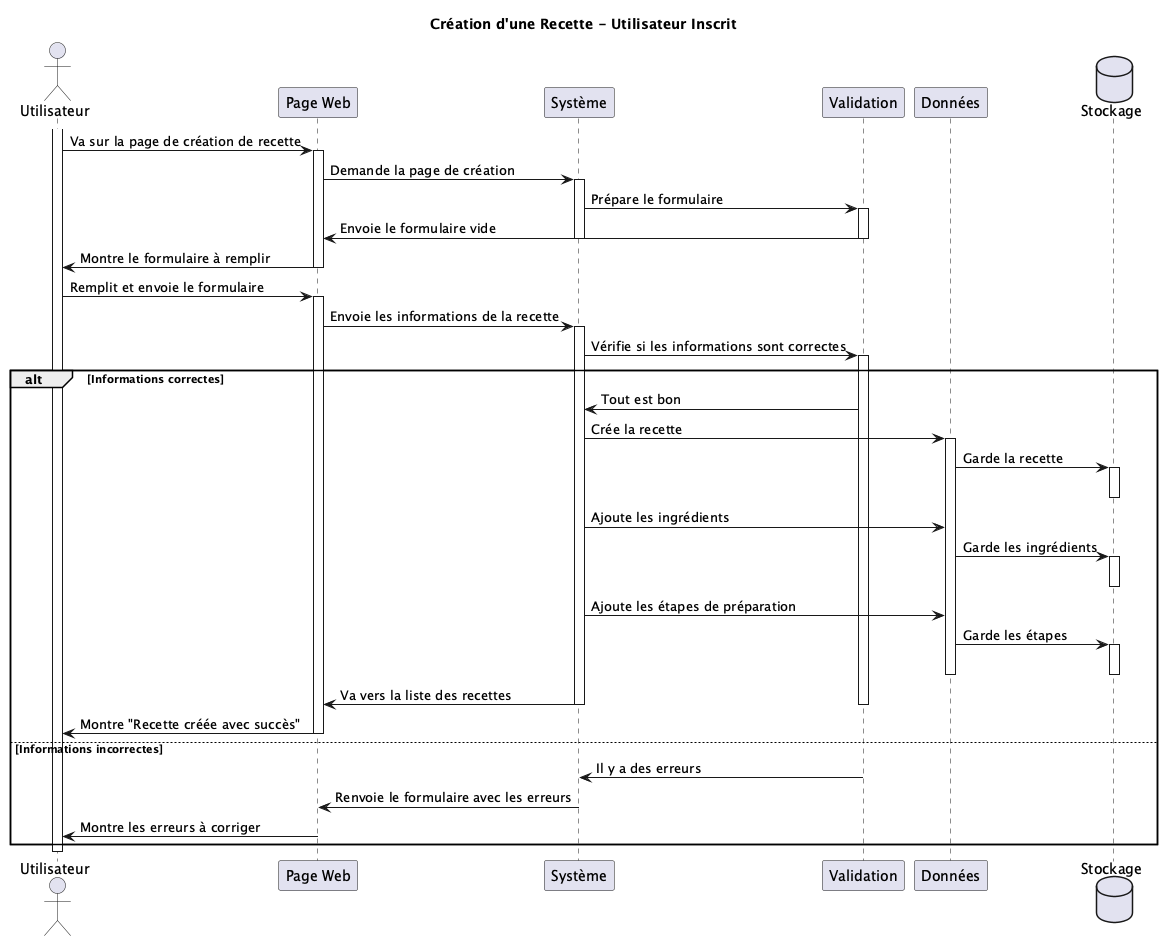
\includegraphics[width=0.95\textwidth]{sequence_diagram_creation_recette.png}
    \caption{Diagramme de séquence – Création d'une recette}
    \label{fig:sequence_creation_recette}
\end{figure}

Ce diagramme illustre le processus complet de création d'une recette par un utilisateur inscrit. Le scénario commence par l'authentification de l'utilisateur qui accède à la page de création de recette. L'utilisateur remplit le formulaire avec les informations de base de la recette (titre, description, difficulté, type de plat, cuisine), ajoute les ingrédients avec leurs quantités et unités, définit les étapes de préparation, sélectionne des tags de catégorisation et télécharge une image. 

Le système valide les données soumises, crée l'objet Recipe en base de données, associe les ingrédients via la table de liaison RecipeIngredient, enregistre les étapes de préparation dans la table Step, et lie les tags sélectionnés. Une fois la recette créée avec succès, l'utilisateur est redirigé vers sa liste de recettes avec un message de confirmation. Ce processus garantit l'intégrité des données et la cohérence des relations entre les différentes entités de l'application.

\subsection{Diagramme de séquence : Création d'un ingrédient}

\begin{figure}[H]
    \centering
    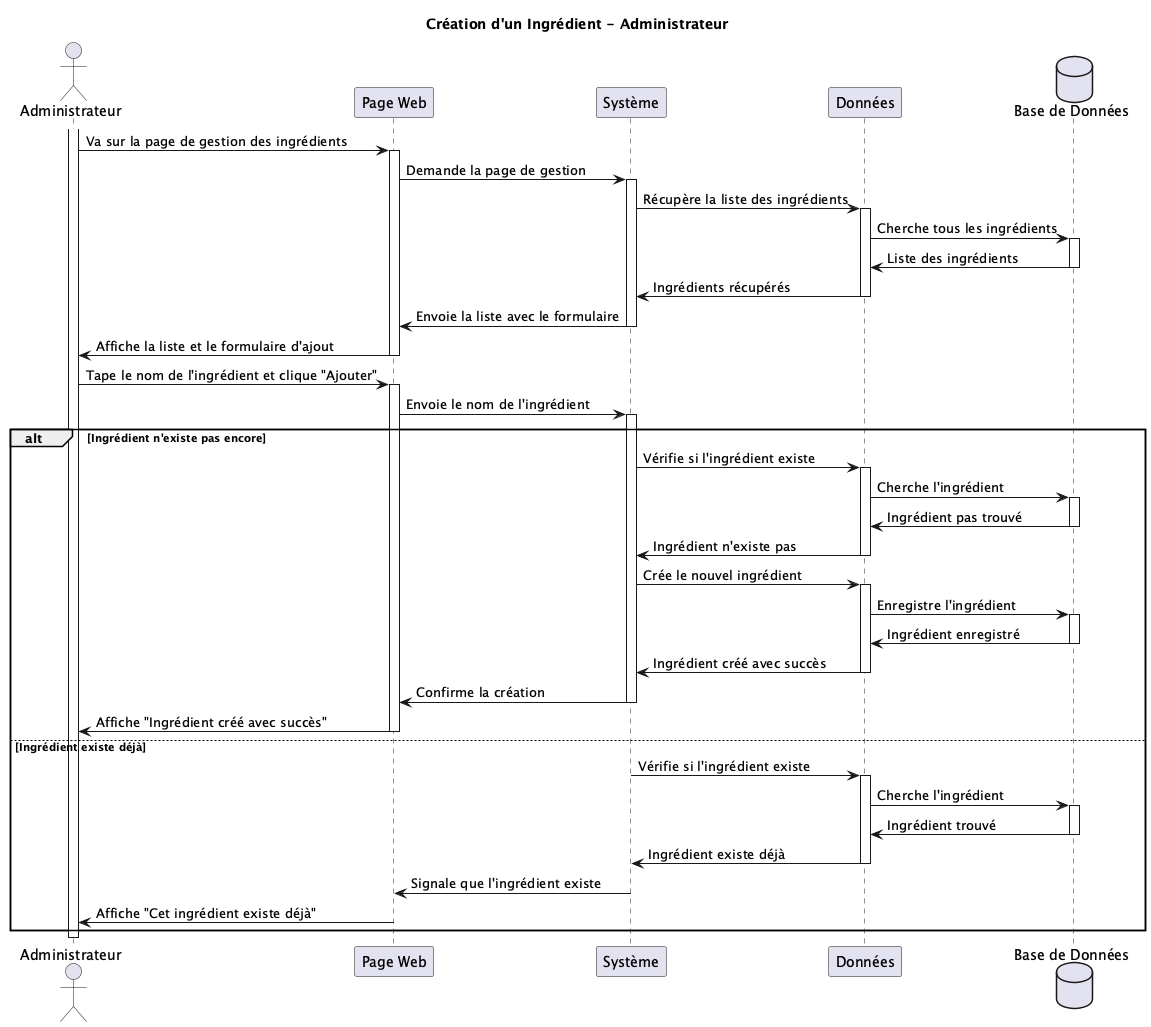
\includegraphics[width=0.95\textwidth]{sequence_diagram_creation_ingredient.png}
    \caption{Diagramme de séquence – Création d'un ingrédient}
    \label{fig:sequence_creation_ingredient}
\end{figure}

Ce diagramme décrit le processus de création d'un nouvel ingrédient par l'administrateur. L'administrateur accède à l'interface de gestion des ingrédients, remplit le formulaire avec le nom de l'ingrédient et sélectionne l'unité de mesure appropriée (grammes, litres, cuillères, etc.). Le système valide les données, vérifie qu'aucun ingrédient similaire n'existe déjà dans la base de données, puis crée le nouvel objet Ingredient.

Cette fonctionnalité est réservée à l'administrateur pour maintenir la cohérence et la qualité de la base de données des ingrédients. L'ingrédient créé devient alors disponible pour tous les utilisateurs lors de la création de leurs recettes, garantissant ainsi une standardisation des noms et des unités de mesure utilisés dans l'application.

\subsection{Diagramme de séquence : Création d'un article de blog}

\begin{figure}[H]
    \centering
    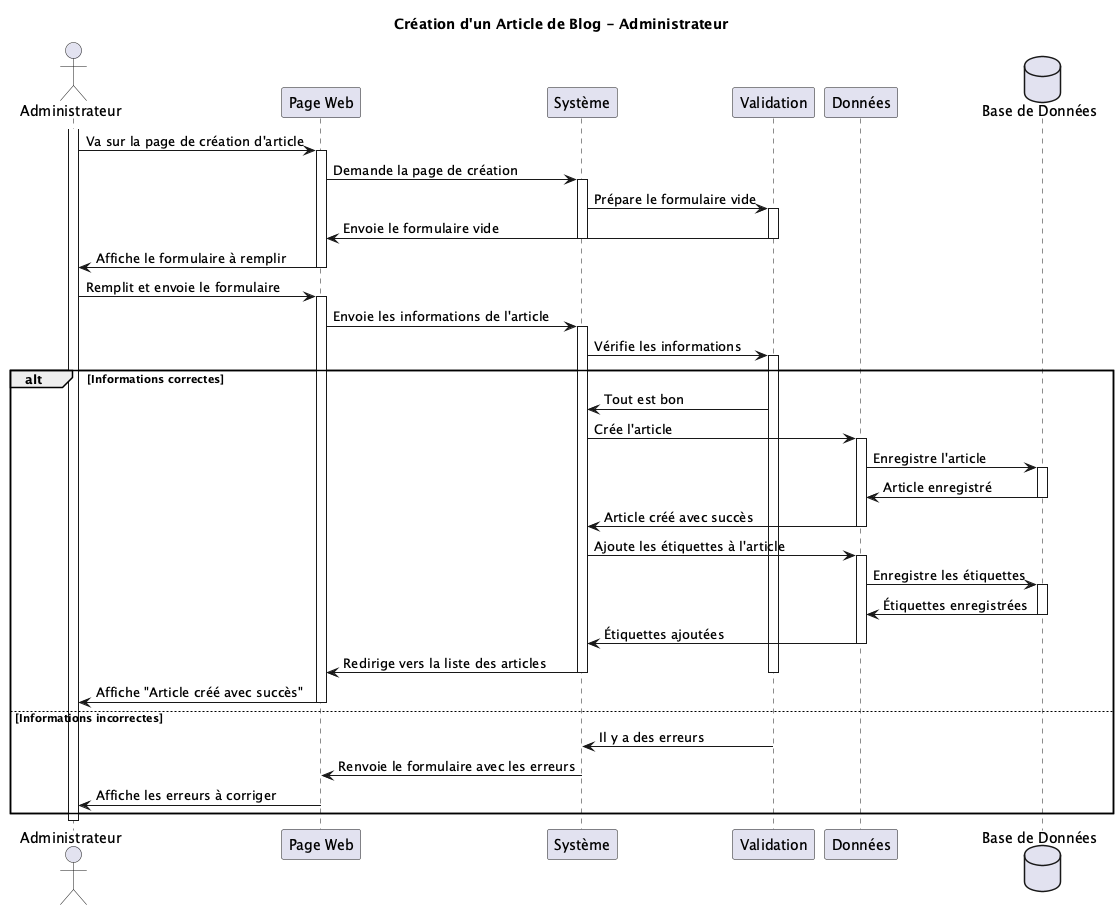
\includegraphics[width=0.95\textwidth]{sequence_diagram_creation_blog.png}
    \caption{Diagramme de séquence – Création d'un article de blog}
    \label{fig:sequence_creation_blog}
\end{figure}

Ce diagramme présente le processus de création d'un article de blog par l'administrateur. L'administrateur accède à l'interface de création d'articles, remplit le formulaire avec le titre, le contenu de l'article, sélectionne des tags de catégorisation et peut éventuellement ajouter une image d'illustration. Le système valide les données, crée l'objet Blog en base de données, associe les tags sélectionnés et enregistre l'image si elle a été fournie.

L'article créé devient immédiatement visible pour tous les utilisateurs de la plateforme, contribuant ainsi à l'enrichissement du contenu culinaire et à l'animation de la communauté. Cette fonctionnalité permet de partager des conseils, des astuces culinaires, des recettes spéciales ou des articles thématiques avec l'ensemble des membres de la plateforme.

\subsection{Diagramme de séquence : Ajout d'une recette aux favoris}

\begin{figure}[H]
    \centering
    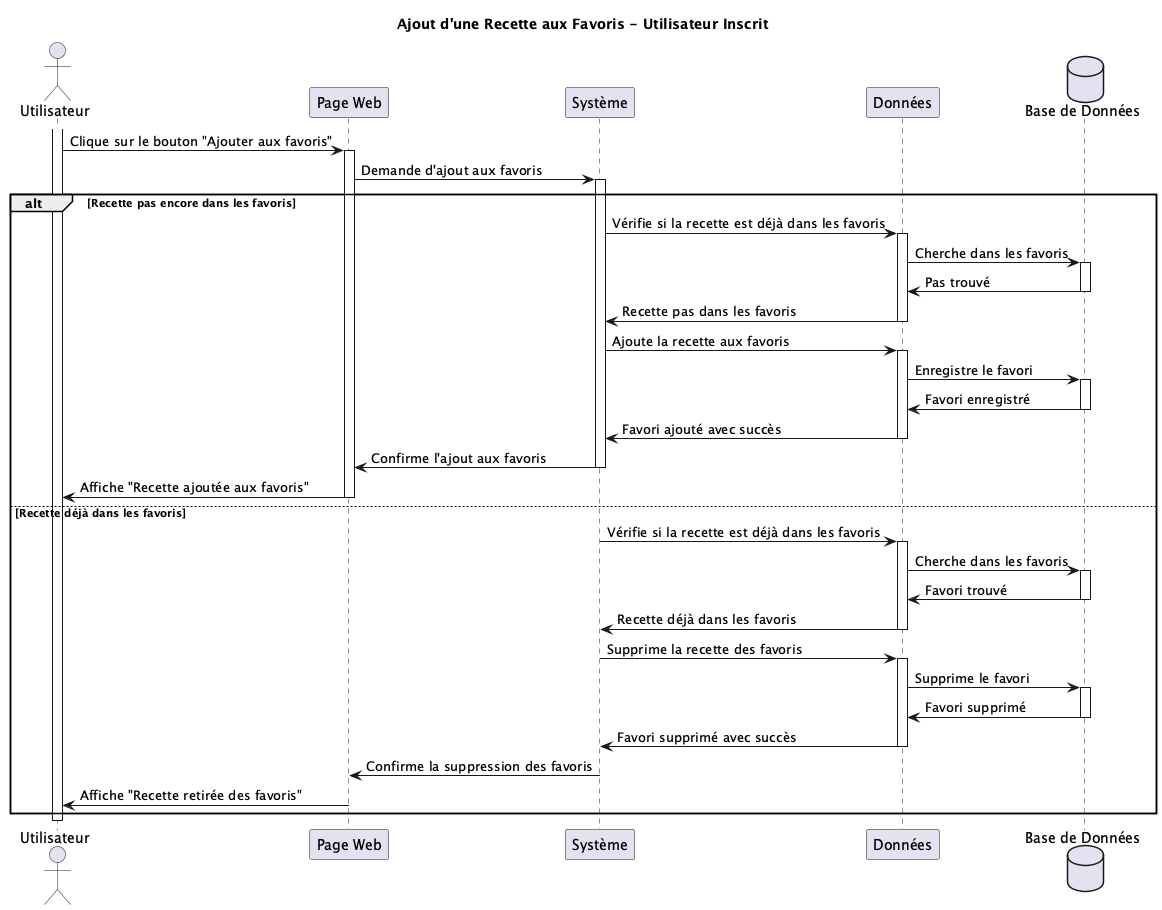
\includegraphics[width=0.95\textwidth]{sequence_diagram_ajout_favoris.png}
    \caption{Diagramme de séquence – Ajout d'une recette aux favoris}
    \label{fig:sequence_ajout_favoris}
\end{figure}

Ce diagramme illustre le processus d'ajout d'une recette à la liste des favoris d'un utilisateur. L'utilisateur inscrit consulte une recette publique, clique sur le bouton "Ajouter aux favoris", et le système vérifie si la recette n'est pas déjà dans ses favoris. Si ce n'est pas le cas, une nouvelle entrée est créée dans la table Favorite, établissant la relation entre l'utilisateur et la recette.

Cette fonctionnalité permet aux utilisateurs de marquer les recettes qui les intéressent pour y accéder rapidement ultérieurement. L'utilisateur peut également retirer une recette de ses favoris en cliquant à nouveau sur le bouton, ce qui supprime l'entrée correspondante de la base de données. Cette interaction simple mais essentielle améliore l'expérience utilisateur en facilitant l'organisation personnelle des recettes.

\subsection{Diagramme de séquence : Ajout d'un commentaire}

\begin{figure}[H]
    \centering
    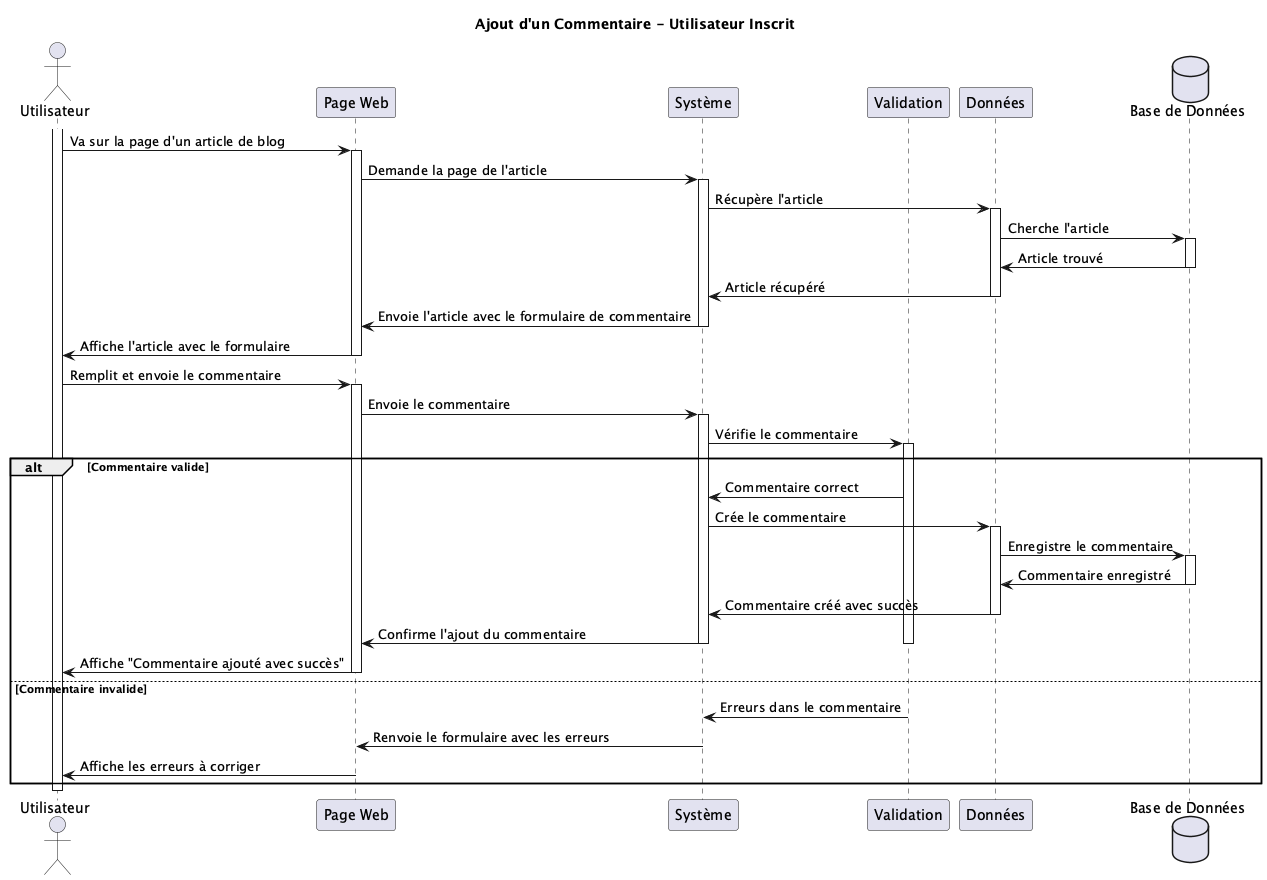
\includegraphics[width=0.95\textwidth]{sequence_diagram_ajout_commentaire.png}
    \caption{Diagramme de séquence – Ajout d'un commentaire}
    \label{fig:sequence_ajout_commentaire}
\end{figure}

Ce diagramme décrit le processus d'ajout d'un commentaire sur une recette par un utilisateur inscrit. L'utilisateur consulte une recette, remplit le formulaire de commentaire avec son texte, et soumet le formulaire. Le système valide les données, crée un nouvel objet BlogComment en base de données, l'associe à la recette et à l'utilisateur, puis rafraîchit la page pour afficher le nouveau commentaire.

Cette fonctionnalité favorise l'interaction entre les membres de la communauté en permettant de partager des impressions, des conseils ou des questions sur les recettes. Les commentaires sont visibles par tous les utilisateurs, contribuant ainsi à l'enrichissement collectif et à l'entraide culinaire au sein de la plateforme.

\subsection{Diagramme de séquence : Export des statistiques}

\begin{figure}[H]
    \centering
    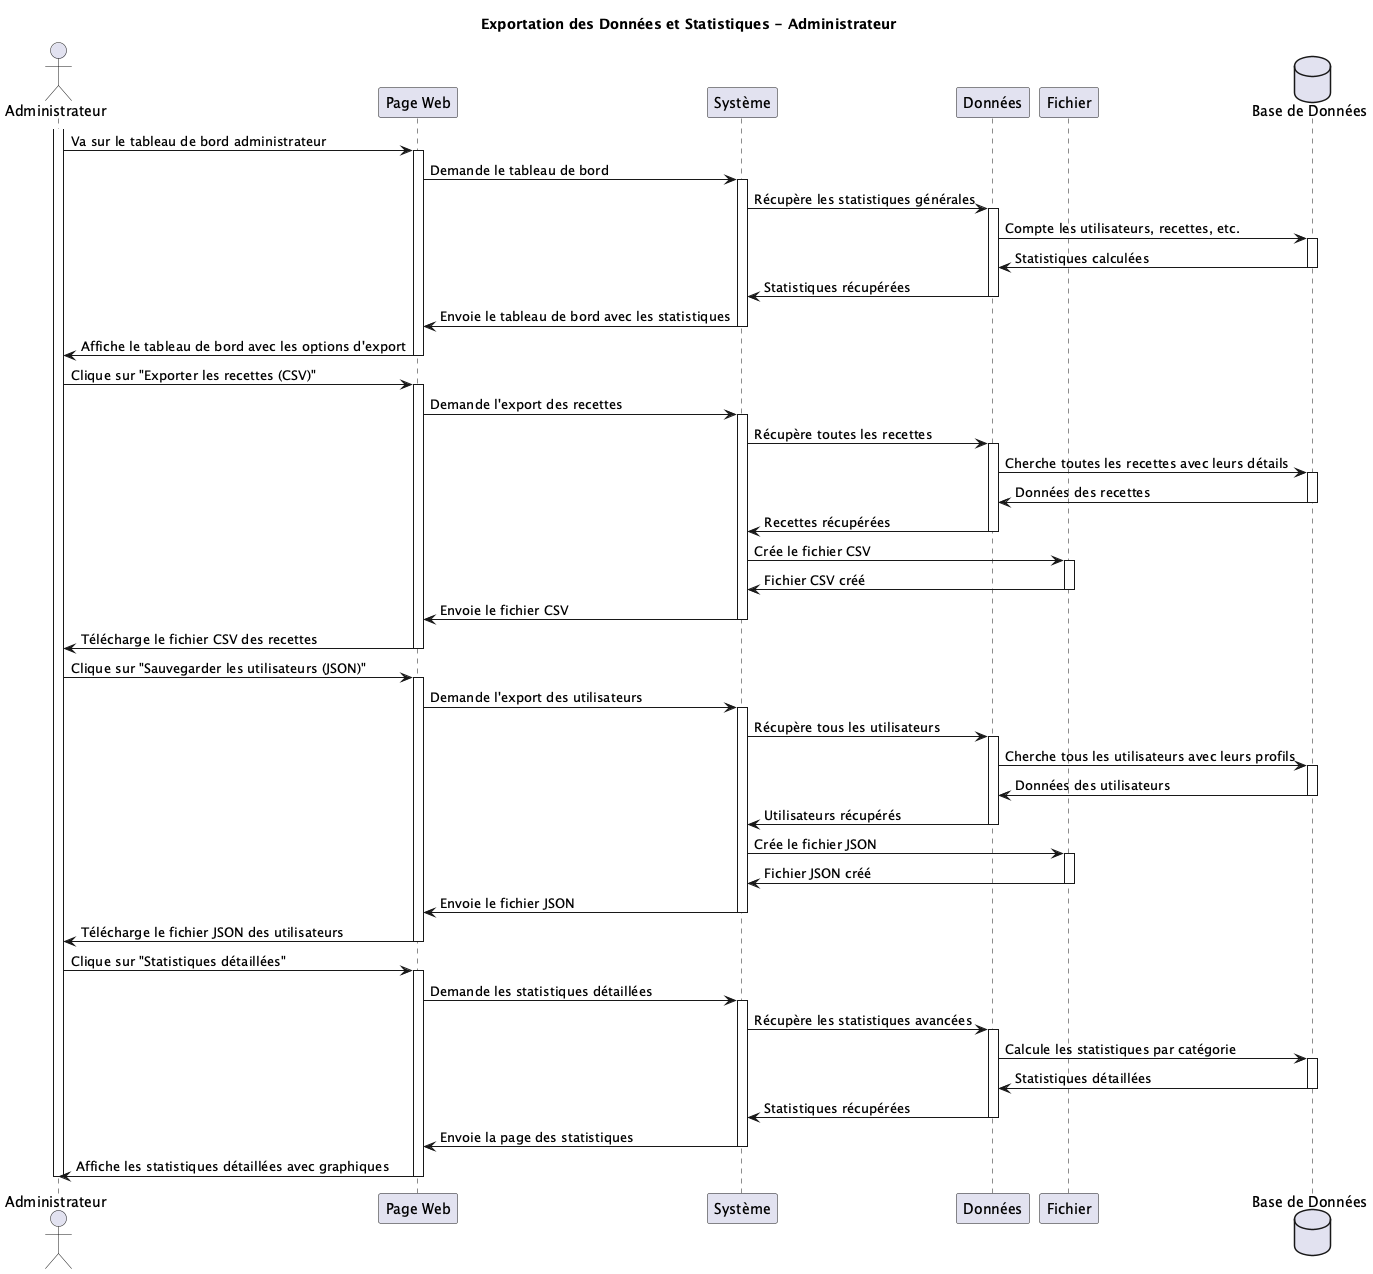
\includegraphics[width=0.95\textwidth]{sequence_diagram_export_statistiques.png}
    \caption{Diagramme de séquence – Export des statistiques}
    \label{fig:sequence_export_statistiques}
\end{figure}

Ce diagramme présente le processus d'export des statistiques des recettes par l'administrateur. L'administrateur accède au tableau de bord d'administration, sélectionne l'option d'export des statistiques, et le système génère un rapport détaillé incluant le nombre total de recettes, les recettes par catégorie, les recettes les plus populaires, les statistiques par utilisateur, etc.

Le système prépare les données, les formate dans un fichier (CSV, Excel ou PDF selon l'option choisie), et propose le téléchargement du fichier à l'administrateur. Cette fonctionnalité permet à l'administrateur d'analyser l'activité de la plateforme, d'identifier les tendances culinaires, et de prendre des décisions éclairées pour l'amélioration et l'évolution de l'application.

\subsection{Diagramme de séquence : Suppression d'un utilisateur}

\begin{figure}[H]
    \centering
    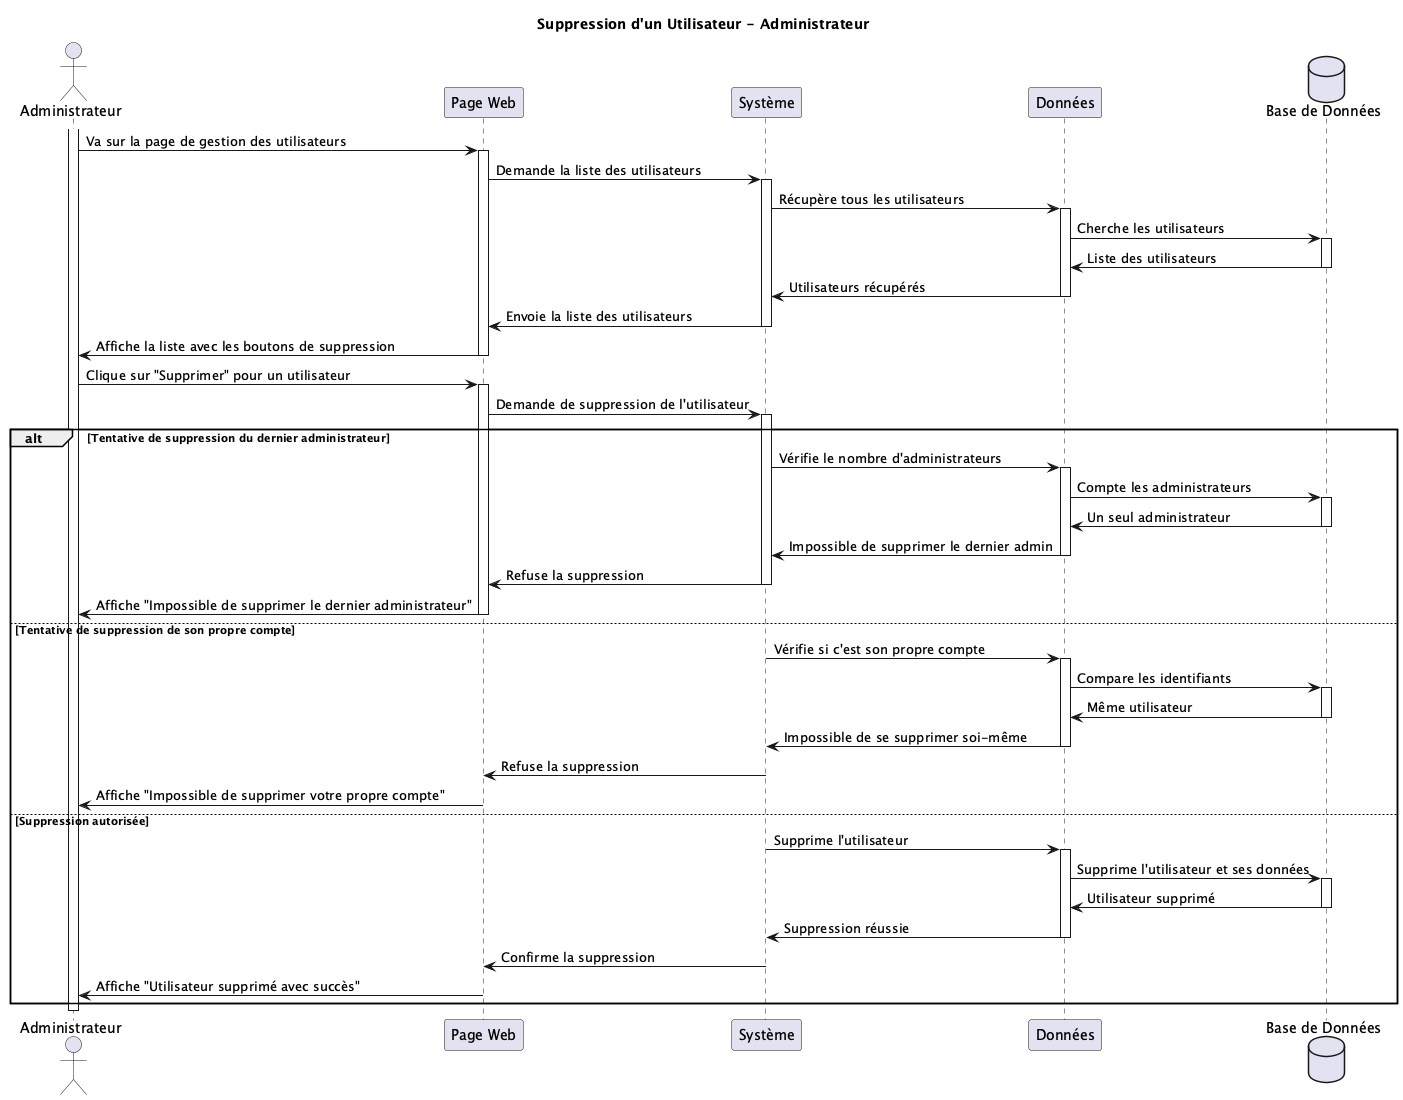
\includegraphics[width=0.95\textwidth]{sequence_diagram_suppression_utilisateur.png}
    \caption{Diagramme de séquence – Suppression d'un utilisateur}
    \label{fig:sequence_suppression_utilisateur}
\end{figure}

Ce diagramme illustre le processus de suppression d'un utilisateur par l'administrateur. L'administrateur accède à la liste des utilisateurs, sélectionne un utilisateur à supprimer, et le système effectue une série de vérifications et d'actions en cascade. Le système supprime d'abord les commentaires de l'utilisateur, puis ses recettes favorites, ses recettes créées (avec leurs ingrédients et étapes associés), et enfin le compte utilisateur lui-même.

Cette opération sensible nécessite des droits d'administration et garantit l'intégrité de la base de données en supprimant toutes les données associées à l'utilisateur de manière cohérente. Le système affiche une confirmation de suppression et met à jour la liste des utilisateurs. Cette fonctionnalité permet à l'administrateur de gérer la communauté et de maintenir la qualité de la plateforme en supprimant les comptes inactifs ou problématiques.

Ces diagrammes de séquence fournissent une vision claire et détaillée des interactions entre les différents composants de l'application lors de l'exécution des principales fonctionnalités. Ils constituent une base solide pour la compréhension du comportement dynamique du système et facilitent la mise en œuvre technique des fonctionnalités décrites.



\section{Diagramme de classes}

Les diagrammes de classes permettent de représenter la structure statique de l’application, en mettant en avant les principales entités (modèles), leurs attributs et les relations entre elles. Voici le diagramme de classes de l’application :

\begin{figure}[H]
    \centering
    \includegraphics[width=0.95\textwidth]{Diagramme de Classe.png}
    \caption{Diagramme de classes de l’application de gestion de recettes}
    \label{fig:class_diagram}
\end{figure}

\subsection*{Description du diagramme de classes}

\begin{itemize}
    \item \textbf{User \& Profile} : La gestion des utilisateurs repose sur le modèle \texttt{User} de Django, enrichi par un profil utilisateur (\texttt{Profile}) qui permet d’ajouter un avatar et des informations complémentaires. Chaque utilisateur possède un profil unique (relation OneToOne).
    \item \textbf{Recette (Recipe)} : C’est l’entité centrale de l’application. Une recette est caractérisée par un titre, une description, une difficulté, une cuisine, un type de plat, des temps de préparation et de cuisson, un nombre de portions, une image, une visibilité (publique/privée), et un auteur (utilisateur). Elle est liée à plusieurs ingrédients, étapes, tags, et peut être ajoutée aux favoris par les utilisateurs.
    \item \textbf{Ingrédients et Étapes} :
    \begin{itemize}
        \item \texttt{Ingredient} : Représente un ingrédient unique dans la base.
        \item \texttt{RecipeIngredient} : Fait le lien entre une recette, un ingrédient, une quantité et une unité.
        \item \texttt{Step} : Décrit une étape de préparation, ordonnée dans la recette.
        \item \texttt{Unit} : Définit les unités de mesure (grammes, litres, etc.).
    \end{itemize}
    \item \textbf{Système de tags} :
    \begin{itemize}
        \item \texttt{Tag} : Permet de catégoriser les recettes et les articles de blog.
        \item \texttt{RecipeTag} : Table de liaison entre les recettes et les tags (relation many-to-many).
    \end{itemize}
    \item \textbf{Favoris} :
    \begin{itemize}
        \item \texttt{FavoriteRecipe} : Permet à un utilisateur de marquer une recette comme favorite.
    \end{itemize}
    \item \textbf{Blog et commentaires} :
    \begin{itemize}
        \item \texttt{Blog} : Module de blog pour publier des articles culinaires.
        \item \texttt{BlogComment} : Permet aux utilisateurs de commenter les articles de blog.
    \end{itemize}
    \item \textbf{Autres entités} :
    \begin{itemize}
        \item \texttt{Cuisine} : Type de cuisine (française, marocaine, etc.) avec code pays.
        \item \texttt{Difficulty} : Niveau de difficulté de la recette.
        \item \texttt{MealType} : Type de repas (entrée, plat, dessert, etc.).
    \end{itemize}
\end{itemize}

\subsection*{Relations principales}
\begin{itemize}
    \item Un \textbf{User} peut créer plusieurs \textbf{Recipe}, \textbf{Blog}, et \textbf{BlogComment}.
    \item Une \textbf{Recipe} est liée à plusieurs \textbf{RecipeIngredient}, \textbf{Step}, \textbf{Tag} (via \textbf{RecipeTag}), et peut être ajoutée à plusieurs \textbf{FavoriteRecipe}.
    \item Un \textbf{Tag} peut être associé à plusieurs \textbf{Recipe} et \textbf{Blog}.
    \item Un \textbf{Blog} peut recevoir plusieurs \textbf{BlogComment}.
\end{itemize}

Ce diagramme de classes reflète la richesse fonctionnelle de l’application et la cohérence de son modèle de données, garantissant une gestion efficace des recettes, des utilisateurs, des interactions sociales et des contenus éditoriaux.
\section*{Conclusion}

% Chapitre 4
\chapter{Étude technique}
\section*{Introduction}
\addcontentsline{toc}{section}{Introduction}
\section{Langages utilisés}
\subsection{HTML / PHP / CSS}
\subsection{MySQL}
\section{Logiciels et Serveur utilisés}
\subsection{Sublime Text}
\subsection{Serveur XAMPP / PHP MyAdmin}
\section*{Conclusion}
\addcontentsline{toc}{section}{Conclusion}

% Chapitre 5
\chapter{Réalisation}
\section*{Introduction}
\addcontentsline{toc}{section}{Introduction}
\section{Interfaces d’accueil}
\section{Interfaces de création}
\section*{Conclusion}
\addcontentsline{toc}{section}{Conclusion}

\chapter*{Conclusion générale}
\addcontentsline{toc}{chapter}{Conclusion générale}

\chapter*{Webographie}
\addcontentsline{toc}{chapter}{Webographie}

\end{document}